\section{方法}
\label{sec:method}

本研究分为两部分：一是对\pol{}文本的要求分析，二是对照这些要求、针对类型化决策模型研究开展的结构化快速证据评估，后者是回答本文政策问题的方法。
在证据评估中，我们在适用之处遵循系统综述和 Meta 分析优先报告条目（PRISMA~2020 声明）~\cite{page2021prisma}与 Cochrane 快速综述指南~\cite{garritty2021cochrane}；流程图与核查清单见\cref{app:prisma}。

\subsection{从条款到要求}
\label{sec:requirements}

我们通读中文文本~\cite{pol2text}及其官方译本~\cite{pol2en}，找出所有要求机器作出判断或对此类判断加以约束的条款，并按其就此类判断所提出的问题对条款进行分组。
由此得到七项要求 G1--G7（\cref{tab:clauses}）。
这些要求是我们对文本的解读，而非文本作者提出的分类。
其中有两处解读选择较为关键。
其一，\clause{4.3.3.1} 要求 PAI 依照框架原则校准其\emph{认知模型}，这属于价值对齐，而非统计意义上的校准；因此，我们将诚实性要求 G4 的依据改置于不在场状态（\clause{4.3.2}）、行为自省（\clause{4.3.3.1}）以及第~7 章的透明义务，这些条款均以所报告的置信度名副其实为前提。
其二，文本并未规定安全阀应如何构建；我们将充当安全阀的类型化模型视为待评估的情形，而非文本所规定之物。

\begin{table}[t]
\centering
\small
\caption{由\pol{}文本导出的要求。条款编号依据提交 \texttt{5791ae3}；所有引文均见\cref{tab:concordance}。}
\label{tab:clauses}
\begin{tabularx}{\linewidth}{@{}l>{\raggedright\arraybackslash}p{0.33\linewidth}L@{}}
\toprule
要求 & \pol{}条款 & 关于类型化保障机制的问题 \\
\midrule
\axis{G1} 检测 & \clause{5.4.1} 安全阀；\art{7}(2)--(3) 异常检测与风险预警 & 能否在部署中依然有效的阈值下，检测违规或越界的内容与行为？ \\
\axis{G2} 可攻击性 & \clause{5.4.1} 安全阀；\clause{4.3.3.1} 恨语截断 & 受审内容能否操纵判定结果？ \\
\axis{G3} 语义公平 & \clause{1.5} 概念并非道德标签；\clause{4.3.1} 平等联结；\clause{4.3.2} 扬爱抑恨；\clause{4.3.3.3} 语义识别 & 判定在选项名称、定义、顺序、措辞、语言与文字变化下是否稳定，在不同群体间是否公平？ \\
\axis{G4} 诚实 & \clause{4.3.2} 不在场状态；\clause{4.3.3.1} 行为自省 & 概率是否经过校准且相互一致？模型能否在应当时报告信息不足？ \\
\axis{G5} 决策链路 & \art{4} 透明与解释；\art{5}(4) 不应是黑箱；\art{5}(5) 可验证的决策链路；\art{9}(2) 解释义务 & 仅为一个数值的判定能否被记录、分解、审计和解释？ \\
\axis{G6} 监督 & \art{9}(7) 非干预原则；\art{10} 争议裁决 & “有把握则执行，无把握则升级”是否可行？升级应止于何处？ \\
\axis{G7} 公共规模 & \art{2}(1) 自治；\clause{5.5} 任何大语言模型都可以纳入治理；\clause{5.6} 逐人评估与公共评估 & 当类型化模型在公众规模上进行判断或模拟时，应满足哪些条件？ \\
\bottomrule
\end{tabularx}
\end{table}

\subsection{纳入标准}

\paragraph{研究。}
我们纳入以类型化决策模型为研究对象、实验组成部分或直接对照的研究。类型化决策模型的操作性定义为：不生成自由文本，而是对调用方声明的选项返回概率分布、或对所声明的陈述返回一个概率的模型。
这涵盖托管的\jev{}、具有相同接口的开源模型，以及生成式模型的类型化读出（当研究将其作为类型化模型处理时）。
首个公开版本的日期须介于 2026 年 9 月 15 日（\jev{}发布之日）与 2026 年 10 月 1 日之间（含首尾两日）。
不限语言和研究设计；非实证条目（评论文章、立场论文、方法说明）予以纳入，但不计入证据计数。
仅提及而未测量或构建类型化模型的论文予以排除，必要时作为背景引用。

\paragraph{灰色文献。}
博客、技术报告和复现代码库在报告了类型化模型的原始测量结果时予以纳入，并以\gmark{}标示。
我们未对其进行系统检索：这些条目来自两个社区追踪列表及下文所述的网络检索。
厂商文档作为背景引用，不计为证据。

\subsection{信息来源、检索与筛选}
\label{sec:search}

我们检索了：
（i）arXiv，于 2026 年 10 月 1 日通过其 API 执行 18 条检索式（\cref{app:queries}），并于 10 月 4 日再次执行，第二次执行旨在捕获较晚公布的论文，但下文的更新检索仍发现了日期在窗口内、而两次执行均未检索到的论文；
（ii）Zenodo，于 2026 年 10 月 1 日通过其 REST API 执行 11 条检索式；
（iii）两个社区追踪列表，即“All about \jev{}”（2{,}073 条记录，其中 52 条标记为论文）~\cite{xiao2026allaboutjev}与\emph{Awesome System One Models}（213 篇经登记核验的论文）~\cite{rafe2026awesome}；以及
（iv）Hugging Face Papers、OpenReview、SSRN 和通用网络检索。
10 月 4 日的 arXiv 检索返回 955 条记录（去重后 606 条），其中 89 条的日期在发布当日或之后；10 月 1 日的 Zenodo 检索返回约 330 条记录，其中 62 条符合关键词与日期标准。经标题、摘要和全文筛选（流程图与计数见\cref{app:prisma}）后，语料库包含 \nArxiv{} 篇 arXiv 论文、\nZenodo{} 条 Zenodo 记录、1 篇仅见于 alphaXiv 的论文以及 \nGrey{} 个灰色文献来源，即 \nPapers{} 项研究与 \nGrey{} 个灰色来源。
其中 \nCoded{} 项报告了与至少一项要求相关的结果，并按下文方法编码（\cref{fig:corpus}）；另有 7 项为非实证条目（评论文章、说明和 1 篇概念性论文），予以记录和评价但不计入计数；其余 22 项为背景层级的工程论文，未予编码。
排除的记录及理由列于 \nolinkurl{data/excluded_records.csv}；10 月 1 日的 Zenodo 筛选仅记录了数量。

\paragraph{更新检索。}
为检验窗口期之后发布的证据是否会改变任何回答，我们于 2026 年 10 月 8 日按照一份书面方案（\nolinkurl{paper/review/UPDATE_SEARCH_2026-10-08.md}）重新执行了检索。
arXiv API 对请求进行了限速，因此同样的 18 条检索式改经 arXiv 的高级检索网页界面执行（\nolinkurl{scripts/rerun_arxiv_search_web.py}）；每条检索式读取一页结果，每页至多 200 条记录，返回记录最多的一条为 91 条（各检索式的命中数见 \nolinkurl{data/search_rerun_2026-10-08_query_hits.csv}），因此没有检索式被截断；不过，网页界面与 API 是不同的检索后端，二者返回的记录未必相同。
11 条 Zenodo 检索式通过 Zenodo API 重新执行（\nolinkurl{scripts/rerun_zenodo_search.py}），两个社区追踪列表则未新增符合条件的条目。
我们全文阅读了 62 个来源；其中 5 个（1 篇 arXiv、4 条 Zenodo）未测量任何类型化模型而被排除，其余 \nUDocs{} 个（31 篇 arXiv、26 条 Zenodo；无新增灰色条目）经过评价：\nUCoded{} 个予以编码（\nUArxiv{} 篇 arXiv、\nUZenodo{} 条 Zenodo），6 个作为背景，2 个为非实证条目，另有 1 个因未评估任何类型化模型而在编码阶段被排除。
在已编码的来源中，\nUSetPostWindow{} 个首次发布于 10 月 2--8 日；\nUSetLateIndexed{} 个是日期在窗口内、但 10 月 1 日和 4 日的检索均未检索到的 arXiv 论文（我们称之为迟索引论文，但无法将索引延迟与检索后端的变更区分开来）；\nUSetReScreened{} 个是日期在窗口内的 Zenodo 记录，构成编码开始后才加入的第三个集合（方案仅列明了前两个集合）。
由于 10 月 1 日的 Zenodo 筛选仅以数量形式记录排除情况，我们无法判断这 \nUSetReScreened{} 条记录当时是被排除还是被遗漏；它们已按相同标准重新筛选，而这一缺口是该次筛选的局限。
合计而言，在日期位于窗口内的 103 项已编码研究中，有 18 项（17\%）仅由更新检索发现，因此主检索的查全率并不完整；按照方案要求，这些研究不计入主计数，\cref{sec:update} 检验将其加入是否会改变任何一项要求的方向。
这 \nURows{} 个研究--要求对采用相同的编码手册和设计评级进行编码，并单独报告（\cref{sec:update}）；主窗口的计数、图表与计票结果保持不变。该方案还冻结了主窗口的确定性评级，规定仅当更新证据改变某项发现的方向或评级时方予更改；这一冻结未被遵守，因为确定性规则在审查期间、即更新研究完成编码之后被修订，所有评级均被重新推导（\cref{sec:appraisal}），这构成对更新方案的偏离。
与主样本不同，每个更新对都由第二位 AI 编码者进行了盲法编码；一致性为 \nUKappaAgree{}（$\kappa = \nUKappa{}$，自助法 95\% CI \nUKappaLo{}--\nUKappaHi{}）。
这是对全部更新对的全量编码，其区间与主样本 $\kappa$ 的区间（\nKappaLo{}--\nKappaHi{}，来自 \nKappaN{} 个抽样对）相重叠，因此两个数值并不能确立二者存在差异；全量编码是对编码手册可重复程度的更好估计。
21 处分歧由已阅读双方理由的第三轮 AI 审读裁定，其中 11 处支持第一位编码者、10 处支持第二位编码者，因此第一位编码者的编码在 \nURows{} 个对中有 10 个被推翻（8\%；\nolinkurl{data/coder_agreement_update_2026-10-08.csv}）；主窗口中位于 \nKappaN{} 个抽样对之外的编码只编码了一次，其中可能有相近比例是错误的。

所发布的编码手册文件（\nolinkurl{paper/review/CODEBOOK_v3.md}）在 10 月 8 日之前缺少本文所陈述的两条规则：一是\cref{app:codebook}的规则（iv），即构成某项要求之检验本身的条件不属于附加条件（自第二轮审查起已载于\cref{app:codebook}）；二是设计较强评级中的独立性条件。
主窗口的主编码者和主窗口的盲法第二编码者（$\kappa = \nKappa{}$）依据的是该文件，并无规则（iv）的文本；更新检索的主编码者被告知该文件包含此规则，而实际上并不包含；更新检索的第二编码者和裁定者则按照本节及更正后文件中的表述应用了该规则。
第十二轮审查中，依照规则（iv）对主窗口全部 G2、G3 和 G6 编码进行的审计，将两个 G3 编码由 Q 改为 N~\cite{arx00831,arx35865}（G3 由 S~2、Q~12、N~10 变为 S~2、Q~10、N~12），G3 的回答“默认情况下并非如此”保持不变。
设计评级始终由脚本按包含独立性条件的规则计算，因此第二个缺口未影响设计评级。

\begin{figure}[t]
\centering
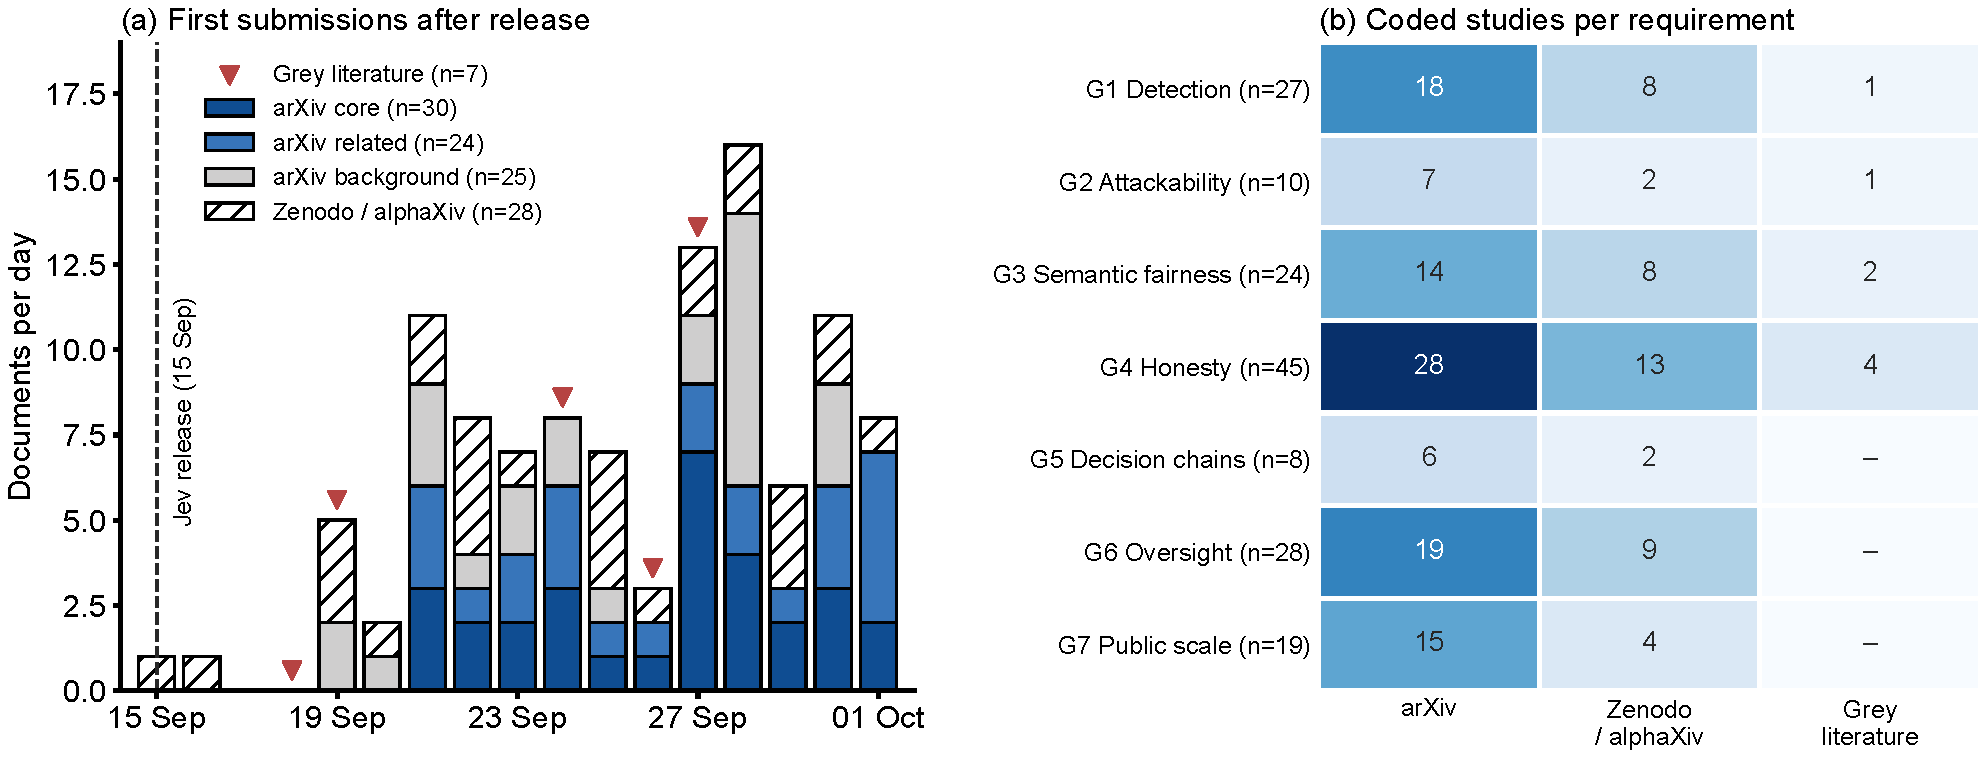
\includegraphics[width=\linewidth]{figures/fig_corpus.pdf}
\caption{证据基础。（a）\jev{}发布后每日的首次投稿：arXiv 论文按层级显示，Zenodo 和 alphaXiv 记录以阴影线表示；三角形标示灰色文献来源。（b）计入计数的已编码研究--要求对，按要求和来源划分；中间一栏含 44 个 Zenodo 对和 2 个 alphaXiv 对，一项研究可涉及多项要求。}
\label{fig:corpus}
\end{figure}

\subsection{数据提取与编码}

对每项研究，我们提取了实际测量的系统（托管的\jev{}、开源模型或二者兼有）、模型版本、任务、数据及其语言、样本量、对照、附有定位信息（节、表或图）的主要结果，以及作者本人陈述的局限。
每篇 arXiv 或 alphaXiv 研究被划入一个层级（\emph{核心}：与某项要求直接相关；\emph{相关}：补充证据；\emph{背景}：工程或其他领域，仅当其报告了与某项要求相关的测量时才予以编码）。
随后，按照对称编码手册（\cref{app:codebook}）对每个“研究--所涉要求”对进行编码，且一律针对\cref{sec:intro}所定义的\emph{检测器}用途：
若主要结果显示类型化模型履行该功能的表现至少与其对照相当，或达到研究自身设定的标准，且无需研究额外附加条件，则编码为\emph{支持}（S）；
若结果显示模型未能履行该功能，或明显逊于其对照，则编码为\emph{不支持}（N）；
若结果不一，或取决于某一附加条件，例如本地拟合的阈值、重新校准、语言或领域限制或人工审查，则编码为\emph{有条件}（Q）。
构成某项要求之检验本身的条件，例如 G2 中的对抗性内容或 G3 中的名称与顺序扰动，不属于附加条件。
对每个已编码的对，我们还记录了类型化模型在该要求上与任何生成式对照的比较结果（更好、相近、更差、不一或无）。
由于各研究的任务、指标和设计不同，我们不合并效应量；综合采用结构化叙述方式，并按 SWiM 指南~\cite{campbell2020swim}所述，对每项研究主要结果的方向进行计票。
编码、附定位信息的理由以及对照比较字段发布于 \nolinkurl{data/evidence_coding.csv}，并列于\cref{app:evidence}；编码计的是研究数量，并非效应量。

\paragraph{一致性。}
第二位编码者在不知第一次编码结果的情况下，仅依据全文和编码手册，对随机抽取的 \nKappaN{} 个研究--要求对进行了编码。
S/Q/N 编码的一致性为 \nKappaAgree{}（Cohen's $\kappa = \nKappa{}$，自助法 95\% CI \nKappaLo{}--\nKappaHi{}）；样本中第一位编码者的编码为 \nKappaMarg{}，因此该样本更多反映的是 Q 与其他编码之间的边界，而非 S 与 N 之间的边界。
两位编码者均为同一模型家族的 AI 智能体，这可能抬高一致性。
四处分歧通过重读原文得以解决，另有一项编码在审查后被修订；所有处理结果均记录于 \nolinkurl{data/coder_agreement.csv} 和 \nolinkurl{data/evidence_coding.csv}。

\subsection{质量评价与确定性}
\label{sec:appraisal}

每项已编码研究按三项条目进行评价：独立性（独立、作者评估自己构建的系统，或与厂商有关联）；设计（预注册；留出评估、交叉验证或重复运行；单次运行；案例研究；非实证）；以及是否报告了样本量和不确定性。
若研究为预注册或留出设计、报告了样本量并附区间或检验，\emph{并且}所评估的系统非作者自建，则评为\emph{设计较强}；若为单次运行、案例研究或非实证，或既未报告样本量也未报告不确定性，则评为\emph{设计较弱}；其余情形评为\emph{中等}，例如报告了样本量但未给出区间的留出研究。
在 \nAppraised{} 个经评价的来源中，\nStronger{} 个为较强，\nModerate{} 个为中等，\nWeaker{} 个为较弱（\nolinkurl{data/quality_appraisal.csv}）。
所有来源均未经同行评审；这一点对所有来源同等适用，因此不作为评级依据。

对于写入摘要或结论的每项发现，我们参照 GRADE~\cite{guyatt2008grade}的思路评定了证据的确定性。
GRADE 将非随机证据的起点定为\emph{低}；基准评测属于非随机证据，我们沿用这一起点。下述降级与升级规则是我们针对单模型基准研究所作的调整，并非 GRADE 本身的组成部分。
若某项发现仅依据单项研究、所依据的研究均非设计较强（例如两项中等研究），或在论断涉及托管\jev{}或一般类型化模型时仅依据开源模型证据，则评为\emph{极低}；若至少两项研究方向一致且其中至少一项设计较强，则评为\emph{低}；若至少三项彼此独立的设计较强研究方向一致，且其中至少一项为预注册或经独立重复，则升为\emph{中等}。包含多个分句的发现，取其各分句中的最低评级。
一项研究只有在以下条件下才计为\emph{独立重复}：其作者与原研究不同；使用自己的数据或重新实现，而非在原数据上重跑原代码；且其设计至少为中等（在原数据上重跑原代码属于再现）；在上述计数中，有共同作者的研究计为一项研究。
每项发现都有其范围，见\cref{tab:keyfindings}：托管\jev{}、开源模型，或一般类型化模型（二者兼有）。证据按系统组计数：同时测试了托管\jev{}与开源模型的研究包含一个托管组和一个开源组，其支持还是反对某项发现，依据被计数的那一组的结果判断。对于关于托管\jev{}或一般类型化模型的发现，评级仅根据托管模型证据计算，即托管\jev{}的研究以及混合研究的托管组；开源模型证据（开源模型研究以及混合研究的开源组）可以佐证此类发现，但不能提高或降低其评级，也不能使其评级有争议。对于关于开源模型的发现，评级根据开源模型证据计算。
这些规则同样向下起作用。若某项研究针对发现所指的系统和情境、就发现所陈述的结果报告了方向相反的结果，则该研究为该发现的\emph{相反研究}；在该结果上兼有两个方向结果的研究，按其主要结果所在的一方计入；超出论断范围的结果，例如论断所指以外的系统、其他结果或论断所排除的情境，既不支持也不反对该发现。
研究按设计评级排序（较强高于中等，中等高于较弱）；在同一评级内，预注册或经重复的研究排在其他研究之上。
任何相反研究都会使该发现被标记为\emph{有争议}；若最强的相反研究的排序不低于最强的支持研究，评级还会下降一级。
对于有关升级的发现，若在同一研究中、在检验升级的任务上，第二阶段比第一阶段更准确，则第二阶段计为\emph{更强的推理模型}；若差异处于抽样误差范围之内，或各准确率指标的方向相反，则视其为同级。
我们将这些规则应用于每一项发现，并纳入所有与之相关的已编码研究，而不仅限于为其引用的研究。凡在某项发现所涉要求上编码的研究，均按系统组列为支持、相反、佐证或不在范围内，并附理由，见 \nolinkurl{data/certainty_evidence.csv}；评级由 \nolinkurl{scripts/rate_certainty.py} 根据该文件与设计评级计算得出，该脚本还核查\cref{tab:keyfindings,tab:certchanges}中列出的评级与其输出是否一致。
\cref{tab:keyfindings} 的最后一个评级行是对照比较编码的计数，而非一组研究，属于描述性内容：该规则不适用于它；我们依判断将其评为低，因为对照比较字段只编码了一次，其一致性未经测量。

这些规则并非最初所采用的规则。10 月 4 日的评级只计入被引用的研究，且该规则无法降低任何评级。该规则在第 12--15 轮审查期间、即更新研究完成编码之后被修订，起因是审查者指出它只能向上起作用、未定义相反研究，且只计入被引用的研究；随后，所有发现均以修订后的规则、基于主窗口与更新检索的全部已编码研究重新评级。由于更新方案冻结了主窗口评级（\cref{sec:search}），这构成对该方案的偏离，\cref{tab:keyfindings} 同时列出 10 月 4 日的评级与当前评级。
10 月 4 日一栏列出的是当日给定的评级。若以当前规则、基于当日引用的研究重新计算，其中一项将为极低（注~$a$）：“预先设定的阈值在新数据上达不到错误目标”当时被评为中等，原因在于为其引用的四项研究中有两项（包括唯一一项预注册研究）测试的是开源模型，第三项在一个数据集上达到目标、在另一个数据集上未达到（\cref{sec:certainty-detail}）。与当日给定的评级相比，一项发现由极低升为低，一项由中等降为低，四项新被标记为有争议；没有发现达到中等确定性，其余评级不变（\cref{tab:certchanges}）。

\subsection{评审者与工具}

本分析由一位作者完成，并大量使用 AI 智能体（所有智能体角色均为 Anthropic 的 Claude Opus 5.5）。
AI 智能体执行了检索，筛选了标题和摘要，从全文中提取数据并附定位信息，提出并应用编码，评价研究质量，担任盲法第二编码者，并由同一模型的新智能体在独立的审查轮次中将正文数字与其来源进行核对；给予智能体的指令、其发现及处理结果均随数据一并发布。
作者确定了研究问题和各项要求，制定了编码手册和判定规则，并对本文的每一项判断负责；在本次发布前，作者未亲自重新编码或逐一复核各项编码。
没有任何人工进行重复筛选、提取或编码，因此未满足 Cochrane 关于由两名人员对至少五分之一记录进行双重筛选的建议~\cite{garritty2021cochrane}。

\subsection{相对于早期发布的变更}

本研究未事先撰写或注册方案。
早期基于摘要的数据集发布~\cite{survey01}未使用编码手册；本分析以全文阅读、对称编码手册、盲法第二编码者、质量评价与确定性评级以及重新执行的 arXiv 检索取而代之，并将一篇未测量任何类型化模型的论文重新归类为背景文献。
